\documentclass[12pt, a4paper, titlepage]{scrartcl}

\usepackage{lmodern}
\usepackage[utf8]{inputenc}
\usepackage[english]{babel}
\usepackage{graphicx}
\graphicspath{{./Figures/}}

\usepackage{url}
%\usepackage{titlesec}
%\newcommand{\sectionbreak}{\clearpage}
\usepackage{dirtree}
\usepackage{color}
\usepackage{listings}
\usepackage{caption}
\usepackage{pdfpages}

%to get clickable links from table of contents
\usepackage{hyperref}
\hypersetup{
	colorlinks,
	citecolor=black,
	filecolor=black,
	linkcolor=black,
	urlcolor=black
}

\newcommand\tab[1][1cm]{\hspace*{#1}}

%\pagestyle{myheadings}
%\markboth{ITI Seminar: Your Name}{ITI Seminar: Your Name}
\usepackage{fancyhdr}
\pagestyle{fancy}
\chead{}
\rhead{}
\lhead{\footnotesize Master Thesis: Institut für Softwaretechnologie - Software Engineering}
\lfoot{\footnotesize Ganesh Ramakrishnan} 
\rfoot{\footnotesize \thepage} 
\cfoot{}
\renewcommand{\headrulewidth}{0.4pt}
\renewcommand{\footrulewidth}{0.4pt}

\newcommand{\courierword}[1]{\textsf{\itshape #1}}{\fontfamily{pcr}\selectfont}%
\setlength{\parindent}{0.0cm}
\setlength{\parskip}{1ex}

\setkomafont{sectioning}{\normalcolor\bfseries}

\title{Continuous Integration in Space Avionics - A Design Using Declarative Build Automation Paradigms\\
\ \\
{\large Master Thesis \\
	Institut für Softwaretechnologie, \\
	Abteilung Software Engineering
\\
%Summer Term 2016
}
}

\author{Ganesh Ayalur Ramakrishnan  \\
  INFOTECH, Universität Stuttgart  \\
  \\
  Supervised by Johannes Lieder \\
  Examiner Prof. Dr. rer. nat. Stefan Wagner
}

%\date{Seminar talk given on \today} 
% \date{Seminar talk given on 25.05.2012}

\begin{document}
\maketitle
%the following is for dedication setting
\iffalse
\newpage \vspace*{8cm}
% Sets a PDF bookmark for the dedication
\pdfbookmark{Dedication}{dedication}
\thispagestyle{empty}
\begin{center}
  \Large \emph{Dedicated to Tamil Nadu farmers, MS Dhoni and Aviationists}
\end{center}
\clearpage
\fi
\textbf{Abstract}
\par There are several benefits when Continuous Integration (CI) is adopted for a software
development project. This provides for a mechanism to prevent human errors during
the build and test of the developed software, as well as help release the product on-time.
Other benefits include capturing errors before they start accumulating, easier integration
at defined intervals over the course of software development, and faster, comprehensive
feedback to developers. However, in an embedded domain, adopting CI is a challenging activity. If the project size and complexity is high, there will be a large number of activities which need to be covered in the CI workflow. Not all tools used in software development provide seamless interfaces to the CI tool. There is a need to design the interface framework which can quickly grow to be complex and time consuming. 
\par An effective CI workflow follows a set of best practices. Build automation is one of them. The existing literature does not provide comprehensive information to address the effect that the build
automation tools have on the design and implementation of a CI framework in an embedded
avionics domain. Tools like GNU Make and Apache Ant are primarily used for the build and
test stages of development. However, these build tools are imperative in nature. As the build logic increases in complexity, the conciseness of build scripts reduces. The build run times should also not be large as the feedback cycle would be longer. 
\par This study aims to design a CI workflow for a space satellite On-Board Software (OBSW) development
project. The objective is to bring out the challenges of using a conventional imperative
build approach during the set-up of a CI framework for the project. The proposal
is to adopt a build tool which is based on declarative build paradigms and provide
for mechanisms to easily integrate with CI tools. This study is carried out as an action research
(AR) with study results expressed as quantitative or qualitative metrics. A prototypical CI chain will be implemented
with a Jenkins CI server and Gradle as the primary build tool. Parameters such as performance, maintenance complexity of build logic, and features such as integration to a CI tool, reproducible builds will be investigated. 

\pagebreak
\tableofcontents 
\pagebreak
\listoffigures
\newpage

\section{Introduction}
\par Software development in embedded critical space avionics is large, complex and expensive. Experience suggests that software problems might result in failed missions. This study is done in collaboration with the department of On-Board Software (OBSW) development, Airbus Defence and Space GmbH in Friedrichshafen. The project under study is the development of central flight software (CSW) which runs on-board a satellite.
\par Software development teams look to maximize value of the product being developed throughout the process lifecycle. Hence, they adopt Agile methodologies\cite{cohen2003agile} which focus on rapid delivery of valuable software through iterative planning and quick feedback loops. This provides several advantages such as easy adaptability to changing requirements, enhanced visibility of the project and on-time release of software. Extreme Programming (XP)\cite{beck2000extreme} has evolved as one of the popular Agile methodologies. XP propagates Continuous Integration (CI). 
\par Continuous Integration (CI) is a practice where developers in a system push to a central mainline several times. The software development environment containing the CI tools and other build tools perform the builds and tests in an automated manner. The developers then expect to receive status of the builds and tests quickly. The CI tool consists of an open source automation server such as Jenkins\cite{jenkinsDoc}. The Figure~\ref{fig:ci-overview-block} shows a global view of the CI concept. A detailed framework definition will be provided in subsequent sections. 
\begin{figure}[!ht]
\centering
\hspace*{-1cm}
	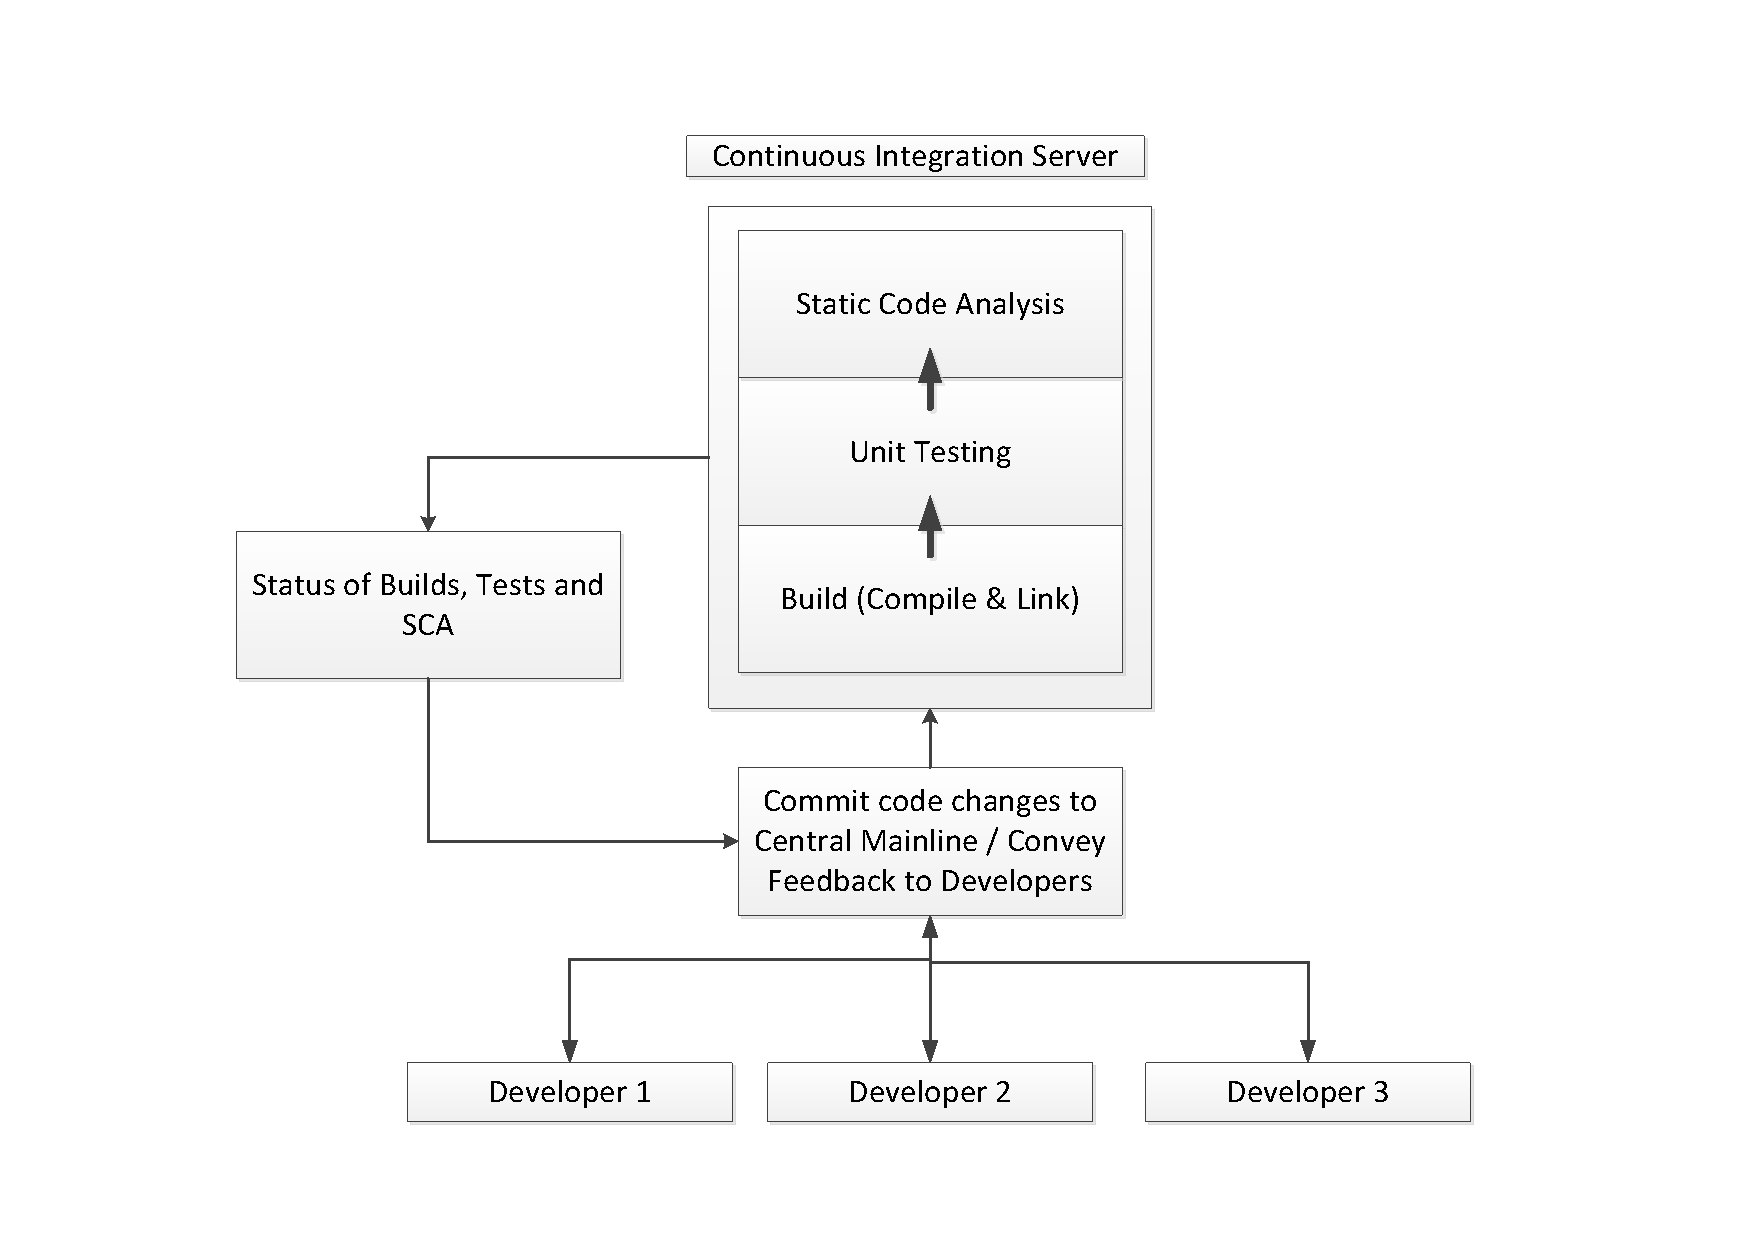
\includegraphics[scale=0.59,clip, trim=0cm 1cm 0cm 1cm]{CI-workflow.pdf}
\caption{Block Diagram to show Overview of CI concept}
\label{fig:ci-overview-block}
\end{figure}
\par The nature of the development project influences the type of CI workflow that the project adopts. For starters, the terminology used in an embedded software development project is slightly different from other development projects. For example, the term build in embedded domain mostly refers to the compile \& link process only. The unit testing is handled separately as is verification \& validation testing. If Git is the version control system in use, then the quality standards on the different types of branches are also quite different. The \courierword{master} could be chosen as the branch which is stable at all points of time. Hence, quality checks at \courierword{master} could be significantly more in number than the other branches. 
\par Continuous Integration (CI) advocates having multiple commits into the central mainline every day. For every single commit, the build is executed from scratch. CI also advocates a higher integration frequency. However, depending on project specific constraints, the development team is allowed to fix the integration frequency. In any case, a team utilizing effective CI model will treat the periodic integration as a non-event\cite{fowler2006continuous}.  
\par The process of automatically creating a software build for a set of source files is called as build automation. It includes activities such as compiling, linking, running unit tests and running quality checks (eg. Static Code Analysis) on the source code. For automating software builds, a large number of tools are available. This thesis incorporates discussion of two such tools, GNU Make\cite{GNUMakeManual} and Gradle\cite{dockter2015gradle}, in detail. In the field of software builds, an \emph{execution unit} (EU) is defined as an activity which the build tool carries out. In Make or Ant they are called as targets. In Gradle they are termed as tasks. Examples for EU's can be compilation of C sources, or cleaning of generated object files for a new build, creation of an executable and much more. Usually, EU's \textit{depend on} other EU's. The build tools also offer a large number of ways in which this dependencies can be configured. A \emph{control flow} is the path which the build tool traverses in a build script to execute the build logic. For example, generation of an executable from C sources involves compilation of the sources, then a stage of link followed by packaging into a binary. Essentially, EU's along with their dependencies combine to define the control flow in software builds. The order of execution of the various EU's may be different and is based on the build author's requirement. Hence, a build script usually contains several targets which in turn means several control flows.  
\par Two important terms that can be associated when discussing build systems are \emph{expressiveness} and \emph{conciseness}. Expressiveness is the capability of the build tool to describe complex build behaviour. Conciseness is when the build tool expresses the build logic in an easy to understand manner. In other words, the control flow of the build logic should be realized by the users of a team without difficulty. More often than not, these properties do not scale proportionately. When build logic tends to become complex, the conciseness of the build script decreases. This trend can be traced back to the build tool that is used to describe the logic. To express this in the form of a graph, consider Figure~\ref{fig:expr-vs-conc}. The traditional build tools such as Make or Ant generally fit into quadrants two or three of the graph. Modern build tools such as Gradle try to be concise at the same time provides opportunity to represent complex build behaviour. Hence, they are slotted in at quadrant four. 

\begin{figure}[!ht]
\centering
%\hspace*{-2ccm}
	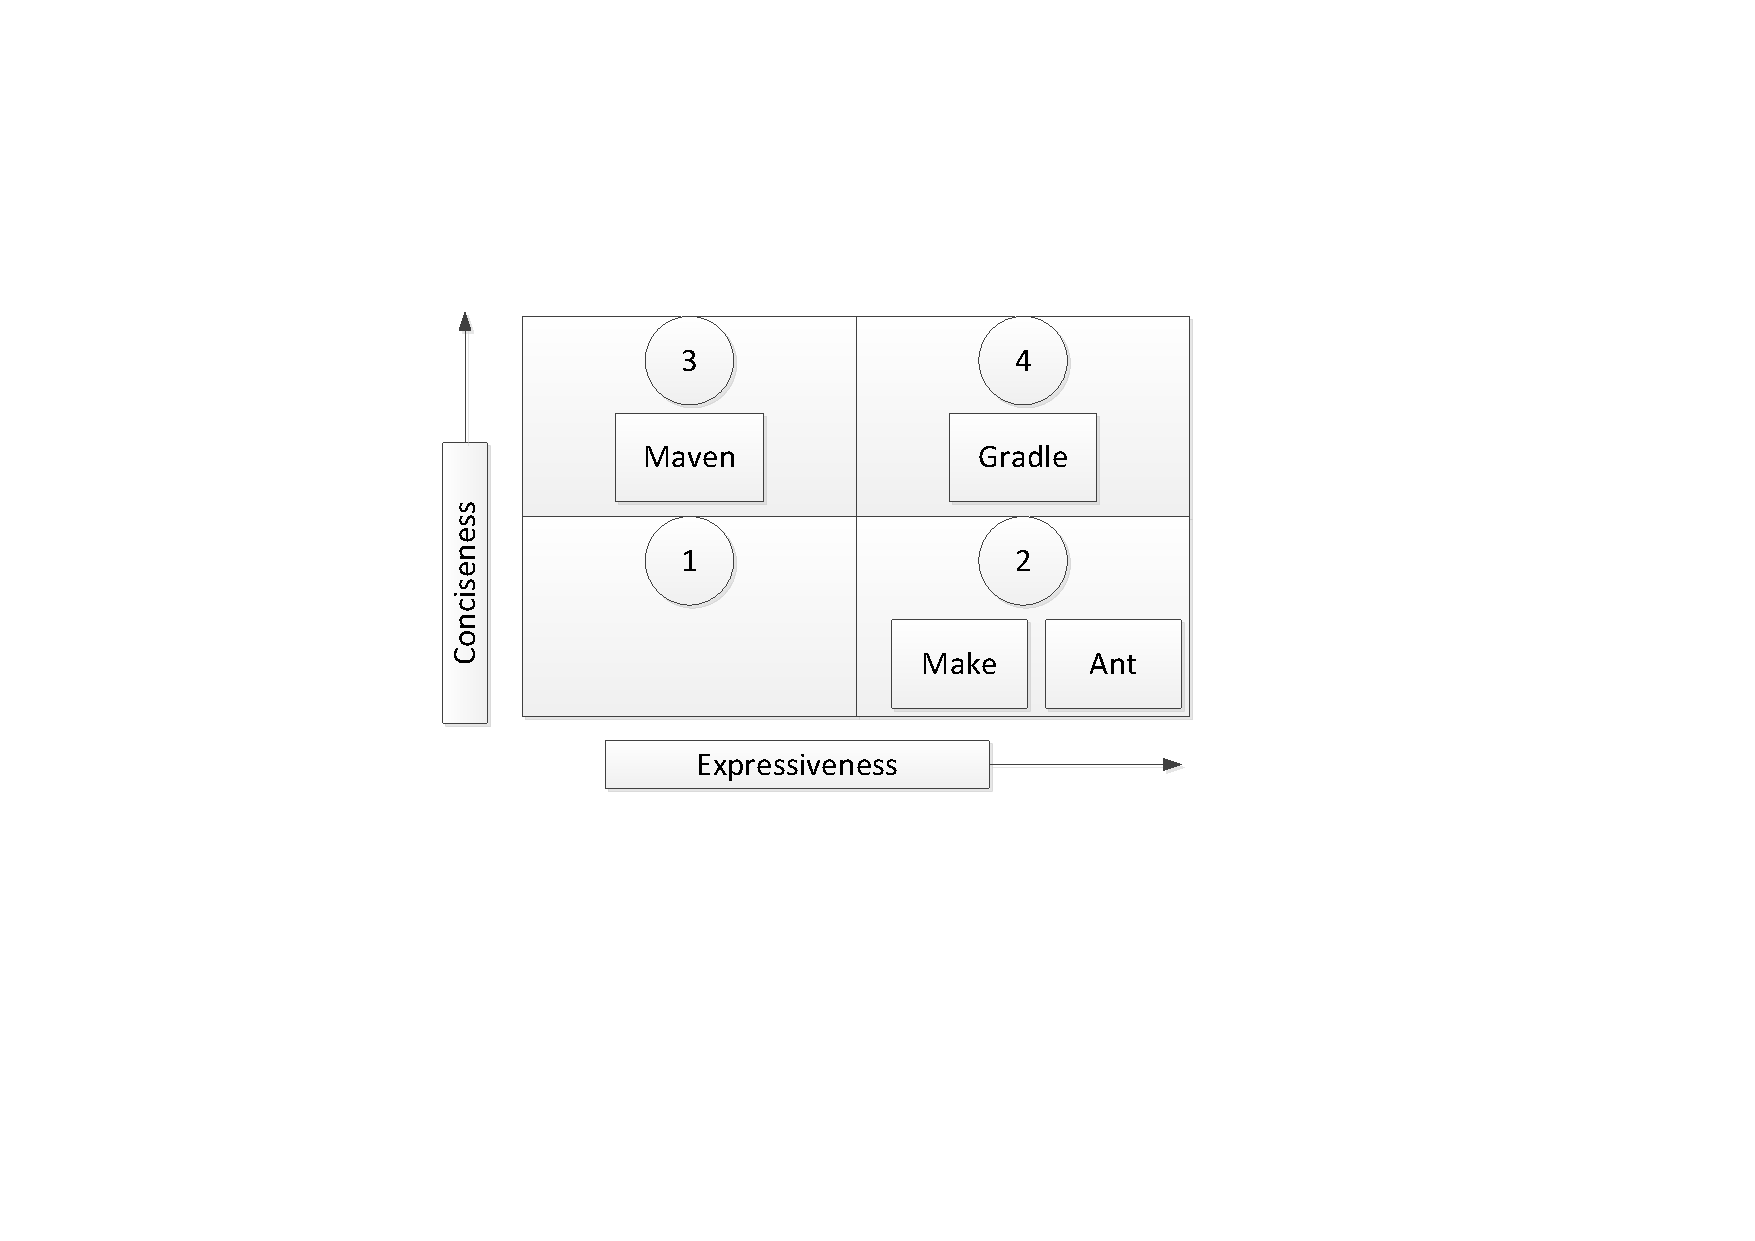
\includegraphics[scale=0.9, clip, trim=6cm 7cm 0cm 4cm]{ExpVsConc.pdf}
\caption{Expressiveness vs Conciseness - How the different build tools fit into this comparison graph?}
\label{fig:expr-vs-conc}
\end{figure}
\par A classification of build tools can be done on the basis of how they are used by the build author. One type is the \emph{imperative} build system. Examples include GNU Make or Apache Ant. This means that it is the responsibility of the build author to define what the build should do and also how the automation tool should do it. In case of a \emph{declarative} build system, the build author is responsible for stating what the build logic should do. The build automation tool attempts to figure out how the requirements are to be met. This convention over configuration approach provided by declarative build systems enable to increase the conciseness of the build logic. 
\par Build automation is generally considered as a CI best practice\cite{fowler2006continuous}. To interface the build tool with a CI tool, a framework needs to designed and implemented. This is called \emph{glue logic}. The implementation of this glue logic is done usually using shell scripting. However, if the build logic is inherently complex, this interface might be difficult to establish and maintain. 
\par This study attempts to provide a method to quantize build systems. This research is implemented as an Action Research (AR). A detailed analysis of the existing build system is done. A discussion with the developers is performed to identify build activities which they commonly use and the challenges that they face with these activities. This initial phase gives rise to a set of observations, opinions and ideas. They are then taken into consideration to form a hypothesis of a new CI framework. A bottom-up approach towards Continuous Integration is done. A CI workflow is created based on the development Gitflow workflow. And the best practices of CI are then applied to this framework. A declarative build tool (Gradle) is used to express the build logic. At the time of design, the developer requirement as well as build design best practices are taken into consideration. A glue logic free system is one of the objectives of this study. This objective is achieved by extending Gradle and leveraging inherent CI tool (Jenkins) functionalities. Better performance is targeted. A reduction in the build-run time can translate to faster feedback and hence on-time release of software. Good software engineering practices are adopted, optimizations are studied, and continuous iterative development is carried out to achieve faster and comprehensive builds. The study also provides a definition for maintenance complexity of build logic when implemented in Gradle. The embedded nature of the project and inherent design methodology of existing build logic are two main factors influencing this definition. Opinions and experiences of the users of the system are taken into account. Additionally, literature covering similar studies are investigated and the knowledge has been incorporated in this study. Thus, the results for measuring complexity that are obtained are a mixture of quantitative and qualitative metrics. Taking the outcomes of these activities, the proposed hypothesis was verified. 
\\
\linebreak
\textbf{Thesis Overview} \\
This thesis is divided into seven sections. Section 2 deals with the background behind the study. It introduces two important components - Continuous Integration (CI) and Build Automation tools. It also provides an overview of the Action Research (AR) methodology on which this study is based. In addition, it describes the Qualitative methods employed in the study. Since this study is performed in an industry, Section 3 provides a detailed report on the context of the software development project in the concerned industry. It describes an overview of the project, the tools used and the workflows adopted. Section 4 explores the Gradle build system which is designed for the project. It covers the terminology used and detailed design descriptions. Section 5 defines the Continuous Integration (CI) workflow designed for the project as part of the study, its benefits and the challenges that were mitigated. Section 6 is an overview of the evaluation done to quantize build systems and the results obtained. Section 7 provides a Summary of the thesis as well as proposes future work that can be undertaken as an extension of this study. 
\pagebreak
\section{Background and Research Approach}

\subsection{Background}
This section provides an overview on two important components of this study - Continuous Integration and Build Automation. 
\subsubsection{Continuous Integration}
\par Kent Beck introduced the concept of Continuous Integration (CI) in its modern style as part of the Extreme Programming (XP) methodology about seventeen years ago\cite{beck2000extreme}. Today, this practice has gained popularity in the field of software development. The practice encourages developers to share their working copies with a central mainline several times a day. The idea is to integrate code often, reduce the workload on the developers post the commit stage and receive frequent and fast feedback of the work. 
\par There are a set of key practices which make CI effective for software development teams\cite{fowler2006continuous}. A few of these practices are handled in this study. 
\begin{enumerate}
\item \textbf{Automate the Build} \\
Build automation is when the source code is converted into a binary such as an executable or a JAR file depending on the type of sources. Several tools are available to perform this conversion. As part of this study, two tools - GNU Make and Gradle will be handled in detail. 
\item \textbf{Every Commit on the Mainline should Build} \\
Another best practice is to test every single commit which is pushed to the mainline. This can be achieved by using a continuous integration server  such as Jenkins. 
\item \textbf{Make it Easy for Anyone to Get the Latest Executable} \\
Additionally, it should be easy for the users of the system to retrieve the executable and use it for their respective needs. Care should be taken to ensure that only the authorized users are capable of getting the executables.
\item \textbf{Everyone can see what is happening} \\
In addition, a good CI design would enable all authorized team members to view the status of the complete system at any point of time.  
\item \textbf{Keep the Build Fast} \\
One primary objective to invest in CI is to receive fast and comprehensive feedback on the status of the build. The framework should be designed to achieve this goal. 
\end{enumerate}
\par The project under study does not have a notion of continuous deployment. Also, it is not a requirement that every member of the team should commit into the mainline everyday. However, every commit that is eventually made should be processed and evaluated. 
\par An effective CI workflow brings about a large number of benefits to the team. There is a possibility to capture errors very early in the life cycle. This would reduce the cost of building the software. A main reason to adopt CI for projects is to not land up in what is termed as an "integration hell"\cite{duvall2007continuous}. This is effectively handled better when integrations are done more often rather than at the time of a release. CI helps to reduce repetitive manual processes. It also provides better project visibility. Developers start to notice trends in the state of their builds and periodically measure quality of the product. There is also an increase in performance leading to on-time releases. Some of these benefits have already been studied and documented in various literature surveys\cite{staahl2013experienced}\cite{miller2008hundred}.
\par On the other hand, adopting Continuous Integration for a software development project can be a challenging activity. There are several articles, case studies and literature reviews which bring out the challenges that teams adopting CI face at the time of development. The nature of the software being developed could influence the CI workflow, especially if the project involves a close relation to hardware\cite{debbiche2014challenges}. If the project size or complexity is large, CI processes need to be thought out with careful considerations. These factors might prolong the release cycles for the project thereby resulting in a slow feedback loop to the team members. 
\par Another important challenge to be considered is the availability of hardware to run the builds. As discussed earlier, the builds need to be fast. And powerful hardware resources help to provide quick feedback of the build runs\cite{claps2015journey}. Software tools provided by the environment in which the build runs also play a significant role towards an effective CI workflow\cite{olsson2012climbing}. A good CI design would constantly strive towards seamless integration of software development tools with the CI framework. 

\subsubsection{Build Systems}
\par This section attempts to describe in brief about the build systems which are used in the project under study. A more detailed analysis of the build logic in the Make based and Gradle based build systems would be discussed later. 
\paragraph{Make}
\par Make is a popular build automation tool which is responsible for creating an executable or a library from source code. It manages to do this by parsing a file called Makefile. Software development of the Make tool started more than 35 years ago\cite{Feldman1979} and there are several variants that are currently available. A very popular and widely used variant is the GNU Make. The format of the Makefiles are similar to one shown below\cite{GNUMakeManual}. 

\noindent\fbox{%
	\parbox{\textwidth}{%
	target : prerequisites \\
		\tab recipe
	}%
}

\par \textit{\textbf{target}} can refer to two things. One is the name of the binary that Make generates. Generally, for C/C++ sources it is an executable or a library. \textit{target} can also refer to an activity which Make carries out like compile, link or clean. \textit{\textbf{prerequisites}} are inputs to the Make system for executing the target. They could be source files, or even other \textit{targets}. A \textit{\textbf{recipe}} is a set of commands which Make carries out. The \textit{recipe} can consist of several commands. By default, a tab space should be included at the beginning of each \textit{recipe} line.
\par The GNU Make build automation tool provides advanced features to enable build author's to describe complex build logic. It provides the concept of implicit rules\cite{GNUMakeManual}. These rules reduce the work load on the build author as it forces Make to use customary techniques for the desired behaviour. For exaple, there are built-in implicit rules which use several Make provided variables in their \textit{recipes} like CFLAGS. There is a possibility to use the Recursive Make\cite{RecursiveMake} functionality. This practice is commonly used when there are separate Makefiles within each subsystem of a larger system. In this case, Make recurses through each of the subsystems and executes the \textit{targets} accordingly. However, the harmful effects of using Recursive Make to software projects is well researched\cite{miller1998recursive}. GNU Make also provides a mechanism to generate dependency information automatically\cite{AutoDepGen}. 
\paragraph{Ant}
\par Ant\cite{ant2004apache} is an open source, software build automation tool similar to Make but targeted primarily for Java sources. It was developed as part of the Apache Tomcat project in 2000. It requires a Java platform, and uses an XML to represent the build logic. The default XML used by Ant is the \courierword{build.xml}. 
\par Each Ant build file consists of a project and atleast one target. Targets are further made up of Ant tasks which can be executed to obtain the desired build behaviour.
\begin{itemize}
\item {\textbf{Project}}\\
Projects are represented in XML using the \textit{\textless project\textgreater}  tag. Three attributes are defined by the Project element. \textit{name} is an optional attribute which denotes the name of the project. \textit{default} denotes the default target for the build script. Any Project may contain multiple number of targets. This attribute defines which target should be executed by default. An optional attribute \textit{basedir} which denotes the root directory for the project. 
\item {\textbf{Target}} \\
Targets are represented using the \textit{\textless target\textgreater}  tag. They are a collection of Ant tasks. They have a \textit{name} attribute and a \textit{depends} attribute. The former defines the name of the target and the latter describes the targets on which the current target depends on. The \textit{depends} attribute defines the order in which the targets are to be executed\cite{williamson2002ant}. \textit{description} is an optional attribute in which a short description for the target can be written. There are also some conditional attributes such as \textit{if} and \textit{unless}.  
\item {\textbf{Task}}\\
Ant tasks are the commands which need to be executed by Ant. Tasks could be similar to an \courierword{echo} command which prints information on the terminal or a \courierword{javac} command which does compilation of the defined Java sources and the classpath. 
\end{itemize}
\par A \textit{\textless project\textgreater} can contain \textit{\textless property\textgreater} element which allows to specify properties such as Ant version, Ant home directory location and much more. 
\paragraph{Gradle}
Gradle\cite{dockter2015gradle} is also an open source build automation tool but replaces the Ant XML build files with a Domain Specific Language (DSL)\cite{van2002domain} based on the Groovy\cite{koenig2007groovy}. It is a tool which provides for a declarative modelling of the problem domain and hence has a build-by-convention approach for software builds. Gradle is already a popular choice for build automation among many enterprises such as Google, Android, and Twitter to name a few\cite{gradleCompanies}. 
\par Gradle defines \textit{\textbf{tasks}} which is an activity carried out during the build such as compile, link or clean. The default name of the build file is \courierword{build.gradle}. Gradle is based on a graph of \textit{task} dependencies, where the \textit{tasks} do the actual work. These \textit{tasks} could be custom tasks created by a build author. It also defines some default \textit{tasks} depending on the configuration that has been mentioned in the DSL. This can be explained with the help of an example.

\begin{figure}[!ht]
\lstset{language=Java,breakatwhitespace=false,
        commentstyle=\color{red},
        breaklines=true, basicstyle=\small\fontfamily{pcr}\selectfont
}
\begin{lstlisting}[frame=single]
apply plugin: 'c'

model {
    components {
        main(NativeExecutableSpec) {
            sources {
               c.lib library: "hello"
            }
        }
    }
}
\end{lstlisting}
\caption{An example of a \courierword{build.gradle}}
\label{fig:gradle-build-file-example}
\end{figure}
\par The first line in Figure~\ref{fig:gradle-build-file-example} includes the \courierword{C plugin} into the build file. This line extends the Gradle project's capabilities. It configures the project based on the conventions described further in the build script. For example, it adds some specific tasks or configures defaults. The Gradle model is a container for configuring the build logic. Based on the DSL specified within the model, Gradle recognizes key configurations and creates a control flow for the build by mapping a set of default tasks which the build author can leverage. For the above mentioned build file, Gradle creates the tasks shown in Figure~\ref{fig:example-task-gradle}. 

\begin{figure}[!ht]
\lstset{breakatwhitespace=false,
        commentstyle=\color{red},
        breaklines=true, basicstyle=\small\fontfamily{pcr}\selectfont
}
\begin{lstlisting}[frame=single]
Build tasks
-----------
assemble - Assembles the outputs of this project.
build - Assembles and tests this project. [assemble, check]
clean - Deletes the build directory.
installMainExecutable - Installs a development image of executable 'main:executable' [mainExecutable]
mainExecutable - Assembles executable 'main:executable'.
    linkMainExecutable - Links executable 'main:executable'
\end{lstlisting}
\caption{The output of \courierword{gradle tasks} command}
\label{fig:example-task-gradle}
\end{figure}
\par The declarative nature of the build tool can be visualized using the above mentioned example. Based on the configuration defined by the build author, Gradle creates the build, clean, install, and link tasks for generating an executable. A detailed study of Gradle's methodology and it's fit in an embedded space avionics software development project will be analyzed in subsequent sections. 

\subsection{Research Approach}
\par The Research Approach used in this study is described. Additionally, a small portion of the results obtained at the end of this study is qualitative in nature. Hence, the practices adopted to bring out qualitative metrics is also discussed in brief. 
\subsubsection{Action Research}
\par Action Research (AR) is a methodology where researchers aim to solve real-world problems while simultaneously analyzing the approach employed to solve the problem\cite{easterbrook2008selecting}. Literature shows that the methodology is cyclic\cite{dick2010action}. There is an intention or a plan to initiate an activity. This precedes action and a stage of review follows as shown in Figure~\ref{fig:ar-cycle}. A prerequisite to Action Research is to have a problem owner who is responsible to both identify a problem as well as take steps towards solving it. There are a large number of key ideas which were developed through an implementation phase in real-world projects\cite{greenwood2006introduction}. One major outcome of AR is an in-depth and first-hand understanding of the subject under study that the researcher obtains\cite{sjoberg2007future}.

\begin{figure}[!ht]
\centering
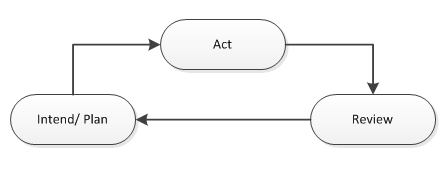
\includegraphics[scale=0.99]{AR.png}
\caption{Action Research (AR) cycle consisting of three distinct stages}
\label{fig:ar-cycle}
\end{figure}

\par AR, when considered as a form of study, also presents challenges to be addressed. Since, AR brings about a notion of change to the project, an alignment with organizational level objectives need to be maintained. Also, the problem of researcher bias at the time of research might be a risk in the study. Finally, the cost of carrying out AR is to be estimated as it could prove to be expensive\cite{easterbrook2008selecting}. 
\par As mentioned earlier, the study of an alternative build automation tool in the field of space avionics to augment to an effective CI workflow is the objective of this study. The researcher in this study is the build author/CI developer. The researcher collaborates with the  members of the software development team to analyze the existing structure of the project. The challenges which need to be mitigated are investigated. In this scenario, the researcher sees this as an opportunity to employ a declarative build paradigm to study first-hand how it would affect the build in an embedded environment. Observations and comments are made during and after development. These observations are then used to either support or refute a hypothesis. 

\subsubsection{Qualitative Metrics in Study}
Quantizing build automation tools is inherently a difficult proposition. This study employs qualitative methods to derive metrics based on a small subset of results. For achieving this, a formal methodology to incorporate these methods into the study is followed. Literature provides starting points to employ qualitative methods systematically\cite{seaman2009using}.  
\par Qualitative metrics provide many advantages to the researcher. Results are richer and informative. Parameters which are hard to be expressed objectively can be explained in a subjective manner. The comments of the developers working on the project are taken into consideration and can be analyzed to offer a concise picture of the state of work.  
\par Qualitative methods involve a phase of Data Collection followed by the phase of Data Analysis. These phases contain different methods for handling data. The methods adopted as part of this study is outlined.
\par \textbf{Data Collection}
\par This study incorporates two different data collection methods. They are \textit{Participant Observation}\cite{taylor1984introduction} and \textit{Interviews}. In \textit{Participant Observation}, the researcher collaborates with the developer in gaining knowledge of the existing system. The developer is encouraged to verbally describe the activities which he carries out so that the researcher is able to understand the process flow. Additionally, the researcher attends the developer team meetings and records key ideas expressed during the meeting. As these meetings are generally organized periodically in a software development team, the researcher is in a position to record data such as terminology used, technical information exchanged as well as identify roles of the developers within the scope of the project. The second technique, \textit{Interviews}\cite{seaman2009using}, is used specifically to collect individual developer opinions and impressions about the subject under study. The researcher has employed a semistructured interview pattern in this study. The interview begins by having specific questions and gradually proceeds towards open-ended questions. The ideas expressed by the developer was recorded by taking notes. This technique of \textit{Interviews} also provide a mechanism for the researcher to capture developer requirements in the study being carried out.
\par \textbf{Data Analysis}
\par Once the data has been collected through the methods described above, an analysis of the obtained data is to be conducted by the researcher. This involves two methods - \textit{Generation of Theory} and \textit{Confirmation of Hypothesis}. Based on the text which is generated by Data Collection, a preliminary processing is done. This processing is called as Coding\cite{wagner2016analysing}. Opinions which are similar or about a particular theme are grouped under a label. For example, consider the following statements made by different team members.\\

\textit{Developer 1 (D1): I would like to find out if this tool would give better performance (faster builds) \ldots \\
Developer 2(D2): The existing system takes about ten minutes to create the executable. If this time period can be reduced, it is a good thing \ldots} \\

Based on the text above, a label called Performance can be introduced. Similarly, different themes can be drawn out from the text and a hypothesis can be generated. 
\par The next method under Data Analysis is \textit{Confirmation of Hypothesis}. Here, a practice called as Triangulation\cite{seaman2009using} is employed. A particular parameter under study is analyzed from various angles. For example, lets consider complexity of build logic as the parameter under study. Qualitative data obtained from interaction with the developers might of the form as: 

\textit{Developer 1 (D1): There are many environment variables in the build logic and I am not sure where they are set \ldots \\
Developer 2 (D2): There are a large number of Makefiles that are included when I run \courierword{make} on my sources. I am not really sure what these Makefiles do \ldots } \\

From a quantitative perspective, literature surveys can help point out measures for complexity of code based on source lines of code (SLOC), or indirection. Hence, it provides an opportunity for the researcher to analyze the parameter from various perspectives. Based on this, it is possible to support or refute the hypothesis that is set. 

\par Most of these methods if not all have been used in this study. Further details of how these methods have aided to help drive the research is discussed in subsequent sections.  

\par This section described about two important components used in this study - Continous Integration and Build Automation. An overview of the research approach used was also provided. The various literature that were a base for this study has also been mentioned at appropriate places. The next section explains the nature of the project under study. 
\pagebreak

\section{On-Board Software Development (OBSW) - AS400 Central Software (CSW)}
The case organization chosen for this study is the Space Systems satellite On-Board Software Development (OBSW) department at Airbus Defence and Space, Friedrichshafen. This chapter provides an overview of the software development activities for AS400 Central Flight Software (CSW) as well as a description of the existing Software Development Environment (SDE) for the same.
\subsection{Overview}
The actual software that runs in an On Board Computer (OBC)\cite{cooper1976development} in a satellite in operation is the On Board Software (OBSW). The OBSW is treated as isolated and independent software controlling the various applications such as power systems, propulsions, sensors and payload on a satellite. The AS400 Avionics development is an initiative towards a detailed definition and development of a generic, re-usable high power avionics system to be used on a variety of missions. 

\subsection{Software Development Environment (SDE)}
\par The term Software Development Environment (SDE) refers to a set of software and associated hardware tools which are used by members involved in the software development project. The environment supports activities such as configuration management, source code development, and project management\cite{dart1992overview}. 
\par The team for building the AS400 Central Flight Software (CSW) is composed of two groups. A production team which provides the flight code and a validation team which performs the validation activities on the provided flight code. The production flight code is in C and the validation test framework is in Java. The SDE that is used by these teams is also composed of two parts. A client side SDE used by developers which consists of development packages in a Windows/Cygwin environment with Eclipse TOPCASED.  And a server side SDE consisting of the Atlassian Tool Suite (JIRA, Stash, Confluence, FishEye, Crucible). A brief overview of these tools is discussed.\\
\textbf{Git:} The version control system used is Git\cite{GitflowWorkflow}. It is a distributed system. Every developer in the team has a working copy in their local machine. They are allowed to 'push' their changes to a central mainline to make it accessible for other users of the system.\\
\textbf{JIRA:} An Atlassian tool which tracks and manages projects\cite{fisher2013utilizing}. It uses an Issue management system. Issues\cite{jiraIssue} are assigned to developers to manage work on different software features as well as other development related activities. \\
\textbf{Stash:} This tool is also a part of the server side SDE. It is responsible for managing the central mainline located on the server. The authorization of the users who are allowed to use the central mainline is well administrated using this tool. A link to JIRA issue management is achieved which maps the development activity to the respective branches in the repositories.\\
\textbf{FishEye }and \textbf{Crucible:} Atlassian tools in the server side SDE. FishEye is used to extract information from repositories, such as code version differences. Crucible is used for requesting, performing and managing code reviews\cite{bacchelli2013expectations}.\\ 
\textbf{Eclipse TOPCASED:} It is the standard Integrated Development Environment (IDE) used by the production team. It is a platform which contains many plugins required for software development. It is a client side SDE tool.
\par As with many embedded applications, this software system is also developed in a cross development environment\cite{rtemsIntro}. This means that the machine on which the code is compiled and linked is different from the actual deployment machine. The former is called as host system and the latter as target. The existing SDE set-up utilizes GNU Make\cite{GNUMakeManual} as the build automation tool and GNU cross compilation tools for the project specific target space processors on the host systems. 
\par Figure~\ref{fig:sde-chart} shows an overview of the SDE used in this project. The blue lines indicate the links between the various applications. The straight black arrows indicate the interface between the team members and the SDE. The developers generally use the cygwin based terminal to push Git commits into Stash. The Issue tracking and Code review activities are generally performed using a web browser. The authorization for the users of this server is managed using Atlassian Crowd which provides integration with the corporate LDAP server.
\par The dotted arrows and the blocks in red are introduced as part of this research. As part of this study, the tools which will be integrated to the existing system are Jenkins and Gradle. Jenkins is an open source automation server which is used for continuous integration. An instance of Jenkins runs on the same server which also caters to the Atlassian Tool Suite. This instance is called as the Jenkins Master instance. The actual build steps are done on so called Slave Machines which are separate Linux based virtual machines. Jenkins receives a hook from Stash when there is a commit into the branches which Jenkins is monitoring. At the end of the build, Jenkins updates Stash with the status. Hence, the developer gets an all-in-one view on the web browser regarding the status of the commit. Clickable links are also provided which enables the developer to open and view the results of Jenkins activities. Gradle is the build automation tool under study which is installed on the Linux based machines as it is here where the build processes are expected to run.
\par One objective behind introducing these features to the SDE is to drive development faster by leveraging the powerful remote virtual machines to automatically build and package the software. The description and set-up of the slave machines and the installation of Jenkins instances are beyond the scope of this thesis. 

\begin{figure}[!ht]
\centering
%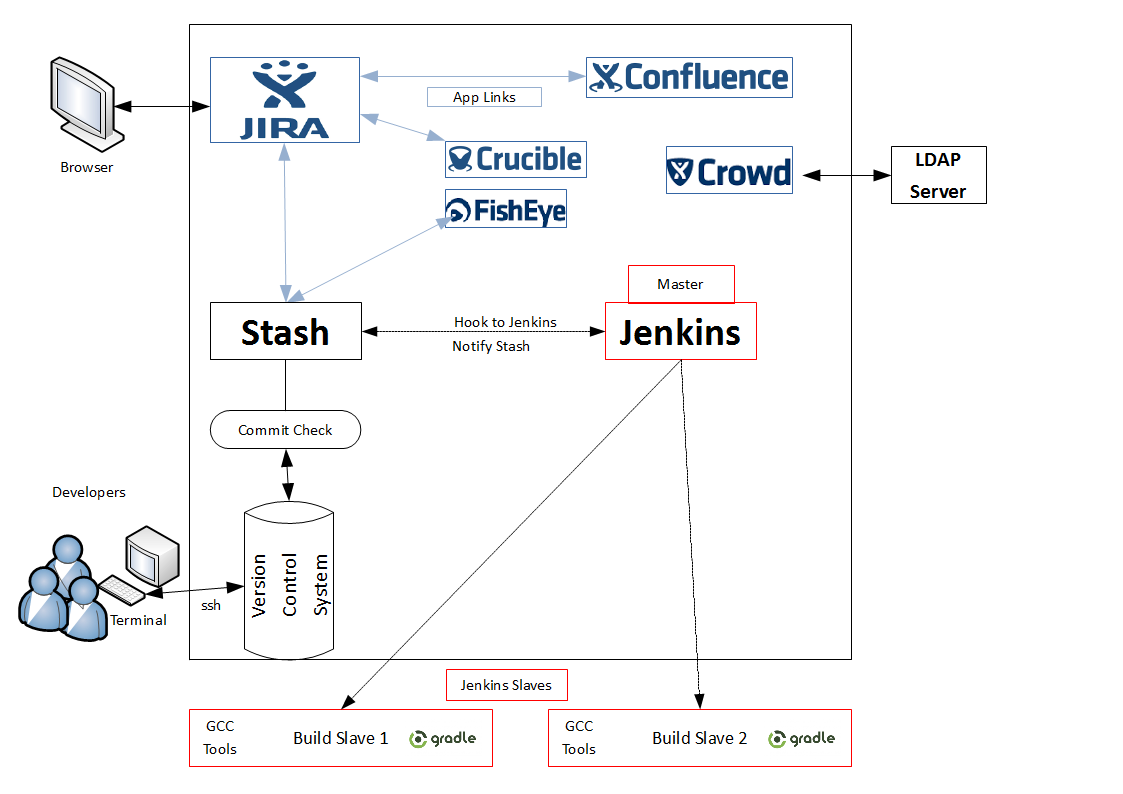
\includegraphics[width=\textwidth,height=\textheight,keepaspectratio]{SDE-Chart.png}
\hspace*{-0.5cm}
	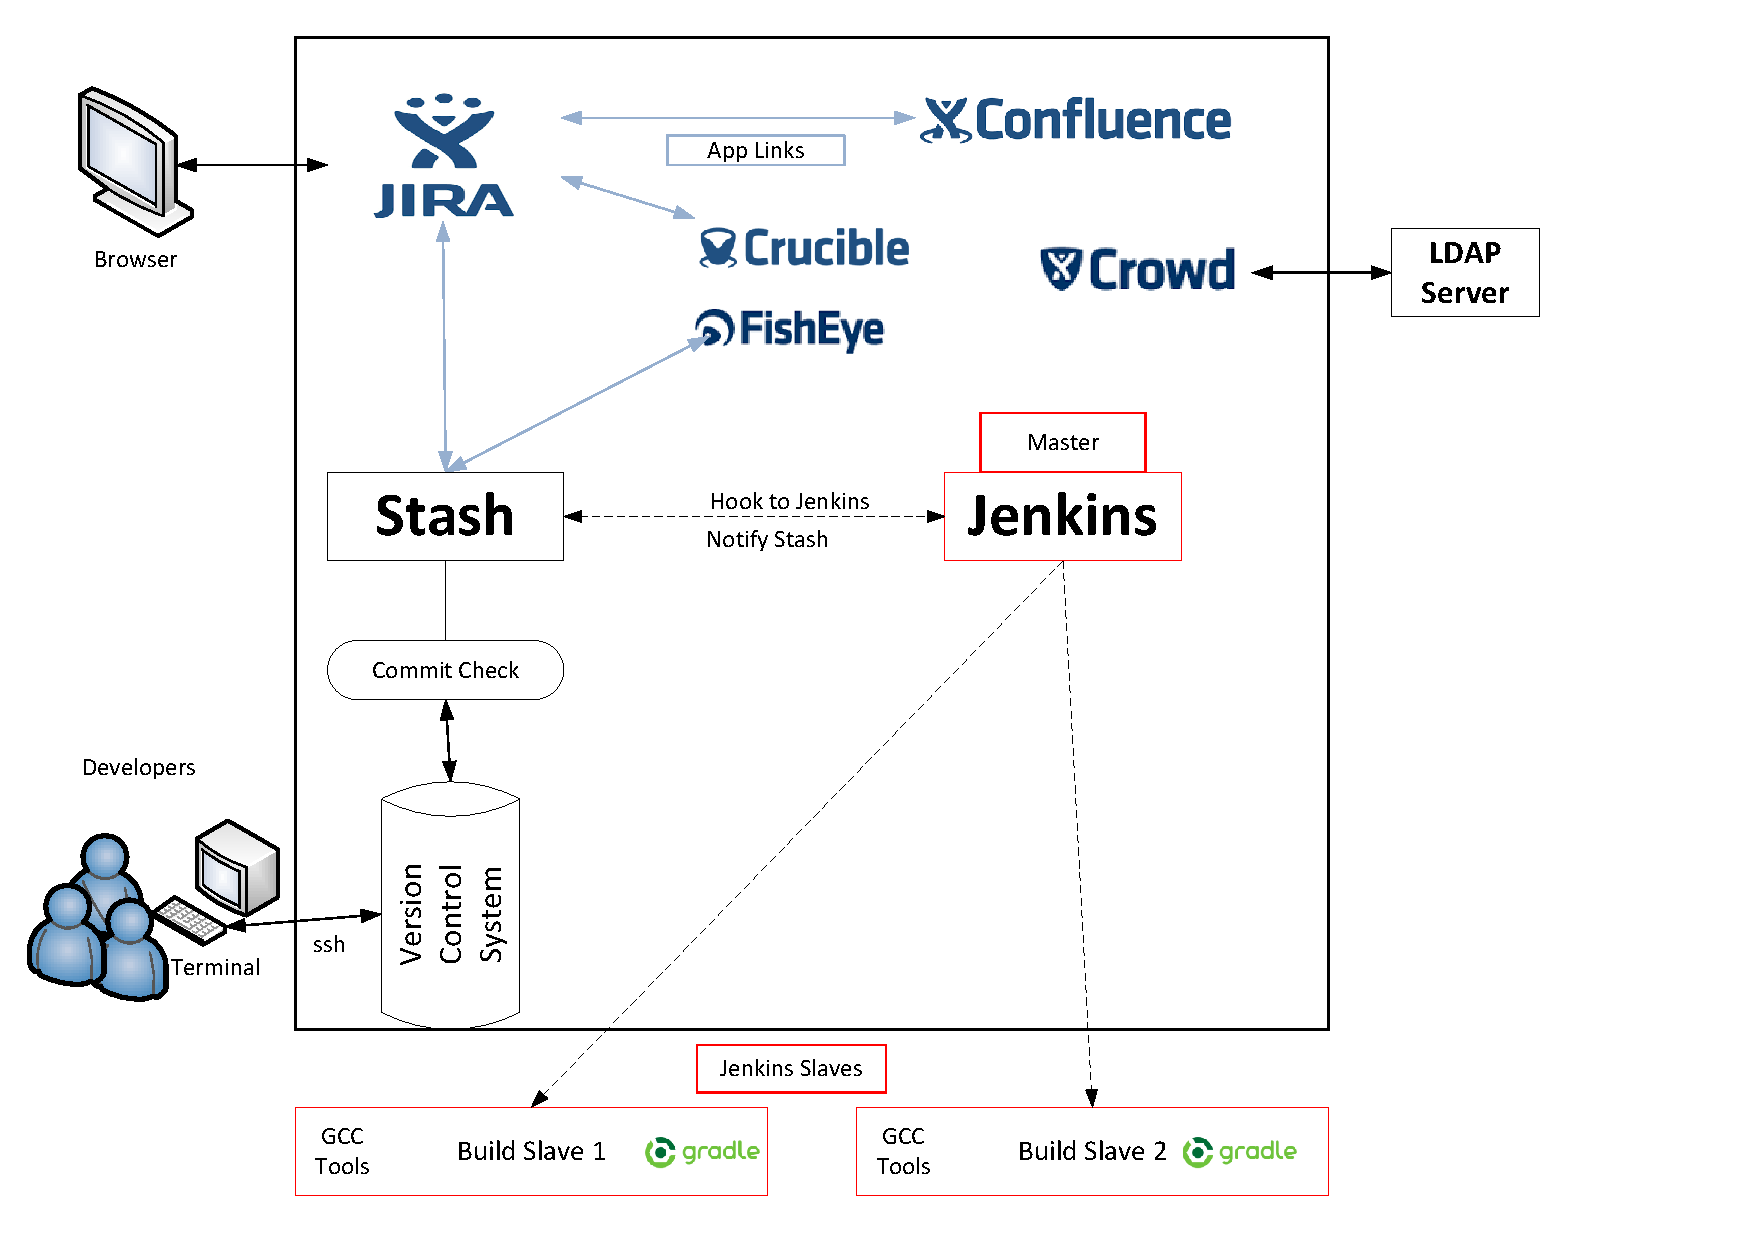
\includegraphics[scale=0.6]{SDE-Chart.pdf}
\caption{SDE set-up for AS400 Central Software Development}
\label{fig:sde-chart}
\end{figure}

\subsection{Software Development in OBSW - CSW}
This section explains the project specific terminology, structure of the source code, git workflow and the build automation methodology employed.
\subsubsection{Terminology}
The source code for the AS400 CSW development is organized as a hierarchy. There are five levels of elements. The top most level is the production repository. The second level contains the different aspects of production such as project specific SDE scripts, source code ('fsw' folder), and libraries to be used in unit testing. The definition of the levels below this need to be distinguished using a view model. This study defines two distinct view models\cite{finkelstein1992viewpoints} for the hierarchy. They are the Developer's view model and the Build Author's view model.
\par \textbf{Developer's View Model}
\begin{itemize}
	\item Applications - they are elements which implement functional processing that are associated with the satellite. Some examples include Data Management System (DMS) which implements data handling standards, and Attitude and Orbit Control Systems (AOCS) which maintains the orientation of the satellite.
	\item Components - Applications can be composed of smaller entities called Components. A typical Component is a function controlling an equipment on board the satellite. 
\end{itemize}
\textbf{Build Author's View Model}
\begin{itemize}
	\item Collections - The elements which are at the same level within the flight software (fsw) folder in the hierarchy are called Collections. They represent the various parts which build up to the Central Flight Software (CSW) Executable.
	\item Constituents - Subordinates of collections which generally contain the source files are called constituents. They usually build up to give the notion of an Application. Some Constituents contain further Sub-Constituents.
\end{itemize}
It should also be noted that Collections do not necessarily map directly towards Applications. Also, it is not mandatory for every Collection to contain Constituents or for every Constituent to contain Sub-Constituents. 

\subsubsection{AS400 CSW Architecture }
As mentioned, the AS400 Project consists of several repositories. Figure~\ref{fig:as400-top-level} shows the various repositories that are used in this study. There are dedicated repositories for production (as400prod) and Validation (as400val). There is also a repository which contains the Make based build logic that is not project specific but shared amongst various related projects. In addition it contains an interface with the SDE for tools which perform Static Code Analysis and Unit Testing. The scripts repositories contain the Glue Logic which creates the interface between the build tools and the CI tools. In addition it contains some helper scripts which allow for integration with Jenkins server. The hierarchy of the production repository is similar to the code tree shown in Figure~\ref{fig:prod-repo-structure}. Some of the Collections within these repositories are git submodules\cite{chacon2011git}. The folders in red are git submodules. The folders in blue are Constituents. The sub-directories within the folder 'fsw' are Collections. This is only an excerpt of the original structure. The actual code tree consists of a larger number of Collections and Constituents. Collections may or may not contain Constituents. The production repository as viewed from the top level of the AS400 Project is self contained.  

\begin{figure}[h]
\noindent\fbox{%
\parbox{\textwidth}{%
\dirtree{%
.1 AS400 Project.
.2 as400prod	-------- Production Repository.
.2 as400val		-------- Validation Repository.      
.2 rtems		-------- RTEMS Operating Systems libraries for link.
.2 SDE			-------- Common Build Logic + SDE Tools.
.2 scripts		-------- Glue Logic for Jenkins, helper scripts, \dots.
}
}%
}
\caption{The AS400 Project top level view.}
\label{fig:as400-top-level}
\end{figure}
\begin{figure}
\noindent\fbox{%
\parbox{\textwidth}{%
\dirtree{%
.1 as400prod.
.2 delivery.
.2 fsw.
.3 aocs           -------------Collection Level.
.4 \color{blue}aocs.          
.4 \color{blue}aocsEquipments -------------Constituent Level.
.5 cbh            -------------Sub-Constituent Level.
.5 str.
.4 \color{blue}aocsMcl.
.3 asw.
.3 boot.
.3 \color{red}dms.
.3 \color{red}infra.
.2 \color{red}sde\_config.
.2 usvf.
.2 uml.
}
}%
}
\caption{An excerpt of the AS400 Production Repository Structure}
\label{fig:prod-repo-structure}
\end{figure}
\subsection{Software Development Workflow}
The AS400 CSW team employs a Gitflow Workflow\cite{GitflowWorkflow} for software development. There are five different types of branches – \courierword{master, develop, release, feature} and \courierword{bugfix} branches. 
\par \courierword{master} contains the official release history. It represents a stable, fully tested release. There is always just a single master branch. Integration of the various software features are done on \courierword{develop}. Generally, there is just a single develop branch. The different features are merged into develop periodically and the team ensures that the required validation tests are done on the commits in develop. 
\par The \courierword{feature} and \courierword{bugfix} branches are used primarily by the developers to work on individual applications. In the organization under study, JIRA issues are called as Software Modification Requests (SMR). The \courierword{feature} branches are created when an SMR is issued. They are usually derived from the \courierword{master} branch.  It is then used by a developer (or a team of developers) to perform the modifications required by the SMR. Commits are made regularly to the branch during development. Ideally, the developers would like to receive fast feedback of the status of their commit when working with \courierword{feature} branches. If the feedback is positive, and if there is a need to merge the contents of the \courierword{feature} branch with the \courierword{develop} branch, the developers can issue a Pull Request\cite{dabbish2012social}. Just ahead of a software release, a new branch called \courierword{release} is forked off from \courierword{develop}.Ideally, this branch is used for bug fixes, documentation generation or other release-oriented activities. When it is ideal for a release, it is merged with the \courierword{master}. 

\begin{figure}[!ht]
%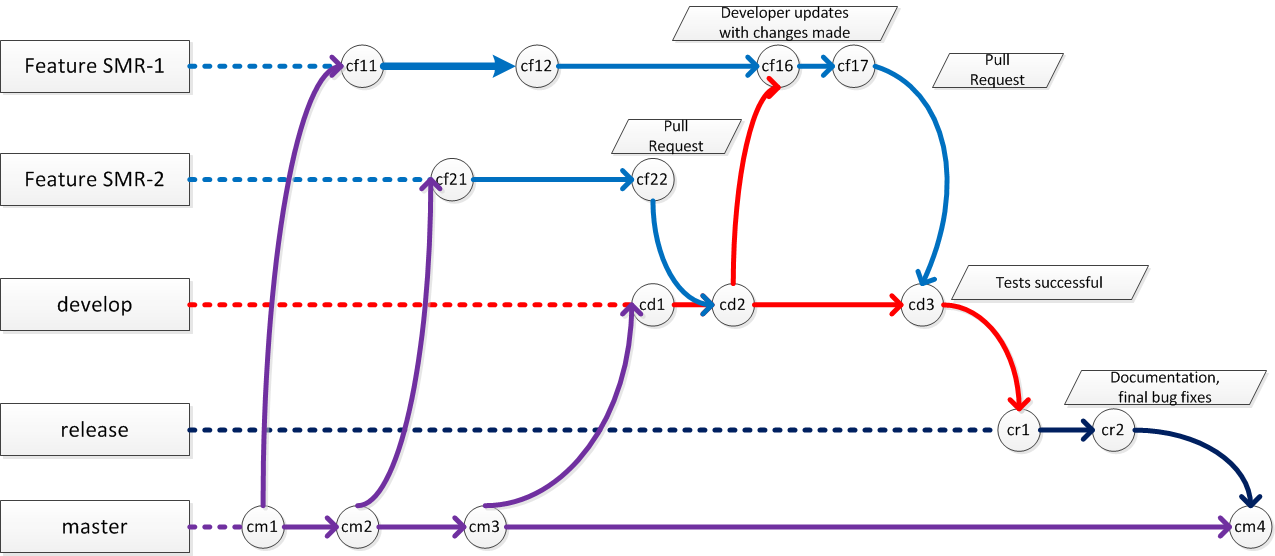
\includegraphics[width=\textwidth,height=\textheight,keepaspectratio]{Gitflow-Workflow.png}
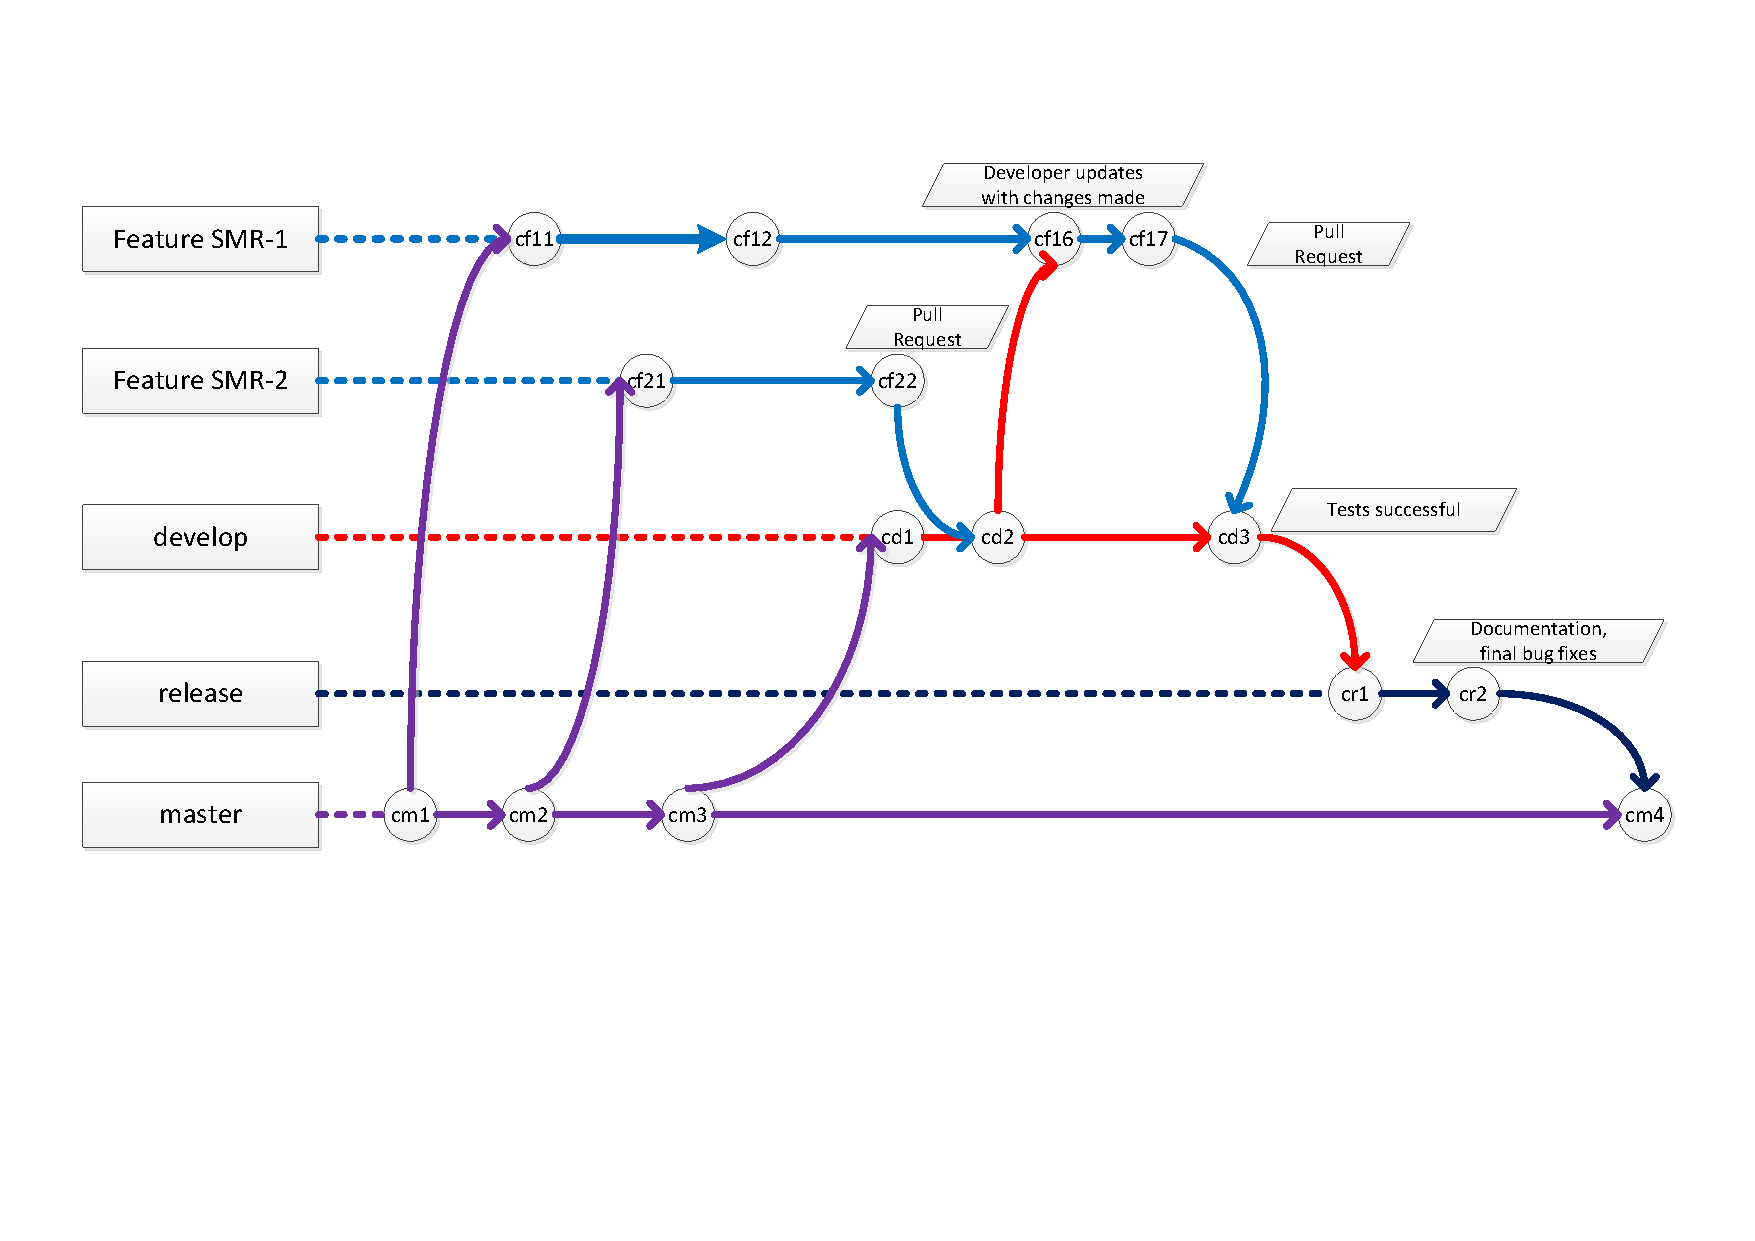
\includegraphics[clip, trim=0cm 5cm 0cm 0cm, width=\textwidth]{Gitflow-Workflow.pdf}
\caption{Representation of the Gitflow Workflow containing master, feature, develop and release branches}
\label{fig:Gitflow-workflow}
\end{figure}%

\par Figure~\ref{fig:Gitflow-workflow} shows an example of how this workflow is used in general by the developers. The developers derive \courierword{feature} branches from the \courierword{master} branch. So \textit{cf11} and \textit{cf21} are the first commits on the \courierword{feature} branches SMR-1 and SMR-2 derived from \textit{cm1} and \textit{cm2} (first and second commits on the \courierword{master}) respectively. At \textit{cf22}, the developer is finished with the work and wishes to integrate with the develop branch. A Pull Request is made and the merge is carried out. The developer working on \courierword{feature} branch SMR-1 now gets the content of \courierword{develop} and continues the work until \textit{cf17}. Another Pull Request is made and the \courierword{develop} is integrated. At a certain point when the \courierword{develop} is ready for a release, like at \textit{cd3}, it is forked off on to a \courierword{release} branch and after final fixes (if required), it is merged with \courierword{master}. 
\par However, for the organization under study, the \courierword{release} branch is used in a different way. At times, \courierword{feature} branches are integrated directly into \courierword{release} before a release. This is done to maintain a record of the different features that were integrated for a particular release. 

\subsection{Build Automation in AS400 CSW}
This section describes in detail the tools and the methodology behind the builds in AS400. In the production environment, the builds for this project are done using GNU Make. In validation, the builds are done within the Eclipse IDE. However, as a headless framework is required for running the builds on remote machines, Apache Ant is used as the build tool. For compilation and linking, GCC tools (part of GNU software) for usage with the RTEMS operating system are used. For Java sources, an eclipse java compiler is used. 
The build system used in the AS400 Project is an inherited system. It has been used previously on successful software projects developed on similar platforms.
\linebreak
\par \textbf{AS400\ Production\ Build\ Process}
\par The next part of this section describes the build logic employed to compile and link the production sources into respective binaries at different points during the build stage. The sources are compiled using Makefiles which are defined in each of the appropriate Collection and Constituent directories within the source code tree. There are also several ‘common’ Makefiles which define variables and rules. The build system uses a recursive Make\cite{stallman1991gnu} model.   
Essentially, the CSW is to be delivered as an executable file. To achieve this goal, the build system uses the technique of Partial Linking\cite{ARMPartialLinking}. Partial Linking generates a relocatable output file which can in turn be used as an input to a linker. It can be achieved easily by appending the \courierword{-r} option to linker arguments. When Partial Linking is invoked, the unresolved references remain unresolved, i.e the errors which a linker raises in normal operation are suppressed. Additionally, this method of linking eliminates duplicate copies of debug sections and merges the symbol table into one. The output of this link stage produces a file which is called as Partially Linked Object (PLO) file.
\par Assume we are considering the AOCS collection in the source tree. It is represented in Figure~\ref{fig:source-tree-collection-constituent}.There are Makefiles within each Constituent and Sub-Constituent directories (in red) as well as within the Collection (in blue). The content of the Makefiles at Collection level and Constituent levels are shown in the Figures~\ref{fig:makefile-aocs} and~\ref{fig:makefile-aocsApFw}. 
\begin{figure}[!ht]
\noindent\fbox{%
\parbox{\textwidth}{%
\dirtree{%
.1 aocs.
.2 aocs.
.3 \color{red}Makefile.
.3 source.c.
.3 header.h.
.2 aocsApFw.
.3 \color{red}Makefile.
.3 source.c.
.3 header.h.
.2 aocsEquipments.
.3 cbh.
.4 \color{red}Makefile.
.4 source.c.
.4 header.h.
.3 gnss.
.4 \color{red}Makefile.
.4 source.c.
.4 header.h.
.3 mag.
.4 \color{red}Makefile.
.4 source.c.
.4 header.h.
.3 mtq.
.4 \color{red}Makefile.
.4 source.c.
.4 header.h.
.3 \color{red}Makefile.
.2 aocsMcl.
.3 \color{red}Makefile.
.3 source.c.
.3 header.h.
.2 aocsMclIf.
.3 \color{red}Makefile.
.3 source.c.
.3 header.h.
.2 \color{blue}Makefile.
}
}%
}
\caption{Source Tree of one of the Collections containing Constituents and Sub-Constituents}
\label{fig:source-tree-collection-constituent}
\end{figure}

\begin{figure}[!ht]
\begin{minipage}[t]{.5\textwidth}
\lstset{language=make,breakatwhitespace=false,xleftmargin=3.4pt,xrightmargin=3.4pt,
        commentstyle=\color{red},
        breaklines=true, basicstyle=\scriptsize
}
\begin{lstlisting}[frame=single][t]
DEFAULT_MAKE = linkpart

# EXTERNAL_LIB : Definition of libraries to use for link, either local to the
#                directory or distant
EXTERNAL_LIB = lib/libaocsApFw.o \
          lib/libaocs.o \
          lib/libaocsEquipments.o \
          lib/libaocsMclIf.o \
          lib/libaocsMcl.o \

LIBDIR = $(OBSW_PATH)/lib

# EXTERNAL_LIB_INST : Definition of libraries to use for link in instrumented mode, either local to the
#                directory or distant
EXTERNAL_LIB_INST =libaocsApFw.o\
          libaocs.o \
          libaocsEquipments.o \
          libaocsMclIf.o \
          libaocsMcl.o \
               
# INCLUDE OF GLOBAL RULES
#------------------------
include $(CPL_REP_MAKE)/Make.rules
\end{lstlisting}
\caption{Makefile for 'aocs' Collection}\par\strut
\label{fig:makefile-aocs}
\end{minipage}%
\begin{minipage}[t]{.5\textwidth}
\lstset{language=make,,xrightmargin=3.4pt,,xleftmargin=3.4pt,
        commentstyle=\color{red},
        breaklines=true, basicstyle=\scriptsize, showlines=true
}
\begin{lstlisting}[frame=single][t]
DEFAULT_MAKE = linkpart

EXTRA_INCLUDE = -I$(AOCS_PATH/aocsEquipments \
                -I$(AOCS_PATH) \
                -I$(DHS_PATH) \
                -I$(INFRA_PATH) \
                -I$(IO_PATH)/busMgr \
                -I$(IO_PATH)/busCplr \
                -I$(IO_PATH)/pmCplr \
                -I$(IO_PATH)/rmapCplr

# SRC : Definition of sources to compile
SRC = AocsApFw.c \
      AocsSync.c \
      AocsAsync.c 

EXTRA_CLEAN = AocsApFwParam.c

# INCLUDE OF GLOBAL RULES
#------------------------
include $(CPL_REP_MAKE)/Make.rules




\end{lstlisting}
\caption{Makefile for 'aocsApFw' Constituent}
\label{fig:makefile-aocsApFw}
\end{minipage}
\end{figure}
\par As this example deals with invoking Make from the aocs Collection level, the process recurses through the various Constituents within this level. Some Constituents like 'aocsEquipments' contain further Sub-Constituents. The invocation also recurses to those levels. The default target defined in these Makefiles will be executed. In this case, it is \courierword{linkpart}. Initially, the sources within the Constituent or Sub-Constituent directories are compiled. For Constituents which contain Sub-Constituents, each Sub-Constituent will then perform a partial link on the generated objects. Constituents which do not contain Sub-Constituents also perform a partial link on its generated objects. This produces a single Partially Linked Object (PLO) file at the respective Constituent or Sub-Constituent level. For Constituents which contain Sub-Constituents, the Makefile at the Constituent Level then performs a partial link on all PLO's generated by the Sub-Constituents. This gives rise to a PLO for that Constituent. Once all Constituents have generated their PLO's, the process now shifts to the Collection Level. The Makefile at the Collection level does the next stage of link. Here all the PLO's produced at its Constituent levels are again partially linked. The build process is so designed that every PLO that is generated is stored at a level higher than the directory in which the \courierword{linkpart} target is executed. This is a common behaviour exhibited by all Collections in the AS400 source tree. As mentioned earlier, as all Collections are located within the 'fsw' directory, all PLO's of the various Collections are written to a 'lib' folder also present within this directory. At the time of generating the complete CSW executable, there is a final link stage where all the PLO's of the different Collections are linked together to produce the software executable. Alternatively, depending on the target defined in a Makefile, the build system also provides for building a static library from the sources. For certain Collections like 'infra', these libraries are used at the final link stage to create the Executable. Hence, it can be observed that three different types of binaries can be obtained - PLO's, executables and Static Libraries. 
\par The build system also provides for building two different variants of the image. The variants differ primarily in the way the sources are compiled. The project defines two distinct database exports which contain several \textit{\#define} directives\cite{stallman1987c} for many identifiers used within the source codes. As these variants represent different configuration settings, the requirements to have two different image variants arises. These image variants are called the SYSDB (system database) and SWDB (software database). The build system allows for generation of these variants based on a command line property \courierword{DATABASE\_DIR}.
\par The project also defines two other variants based on the platform for which the sources are compiled. They are the SCOC3\cite{koebel2010scoc3} and native PC. It should be noted that not all sources in the tree can be compiled for PC. A good example is the 'startup' Collection which contains assembler sources. Hence, the notion of a complete CSW executable for a PC does not exist. However, in the realm of Unit Testing, the compilation for PC platform is  important for capturing bugs. For producing variants depending on the platform, different tool chains are used. For SCOC3, the GNU sparc-rtems compiler and linker are used while for PC the native GNU compiler and linker packages are used. The existing build systems allows for generation of these variants also based on a command line property \courierword{CPU}.
\par In addition to compilation, partial link and link, the build system provides targets for several other activities such as Static Code Analysis, Clean, Linecounter, and Code Instrumentation. The scope of this study does not cover all these targets comprehensively. However, some of these targets are handled and documented wherever applicable. 
\par Now, let us analyze the Makefiles in Figures~\ref{fig:makefile-aocs} and~\ref{fig:makefile-aocsApFw} . Each of these Makefiles includes the ‘common’ Makefile which is called Make.rules. It is like a root Makefile which defines and describes the targets used in these Makefiles. As shown in the figure \courierword{linkpart} is the default target in both these Makefiles. The activity carried out in these Makefiles is partial linking. In the Constituent's Makefile, the variable SRC determines the sources that need to be built. The EXTRA\_INCLUDE variable adds a set of paths which the compiler traverses through to find the include headers for the sources. In the Makefile at Collections level, the EXTERNAL\_LIB variable defines various partially linked objects which need to be sources to the linker. The LIBDIR variable defines the directory to which the output of the link process would be written to.
\linebreak
\par \textbf{AS400 Validation}
\par The validation activities on AS400 CSW is discussed next. OBSW development requires careful and comprehensive validation activities to ensure that the correct software is delivered. For Validation activities, the AS400 team uses a Software Validation Facility (SVF)\cite{hjortnaes1997software}. It is a software test bench which provides a simulated model of the environment where the software is expected to run. It is considered as an hardware-in-loop emulation system as it contains a copy of the target space processor. For the project under study, the SVF is offered by an external team as a package which can used at the time of compilation of test sequences. Several versions of the SVF are released at various points in the software development and the validation team incorporates these changes appropriately. 
\par All the sources required for validation are contained within the repository 'as400val'. The validation framework for this project is in Java. An Eclipse based IDE is used by the validation team members to build and run their tests on the generated CSW Executable. The validation tests contain several Collections based on the Applications to be tested. These Collections contain test sequences in Java. These validation test sequences require test classes developed by the team as well as the SVF packages in the classpath during compile time. Hence, a JAR file containing all these required classes is prepared. For the purpose of a headless build of this JAR, an Ant build xml is created. This is similar to the one shown in Figure~\ref{fig:build-xml-validation}.

\begin{figure}[!ht]
\lstset{language=XML,
		commentstyle=\color{red},
		keywords=\color{blue},
		breaklines=true,
    	basicstyle=\scriptsize,
    	morekeywords={xml, version, encoding, project, target, property, mkdir, javac, classpath, jar, copy}
}
\begin{lstlisting}[frame=single][t]
<?xml version="1.0" encoding="utf-8"?>
<project>

    <property environment="env"/>
    
    <property name="build.compiler" value="org.eclipse.jdt.core.JDTCompilerAdapter"/>

    <target name="clean">
        <delete dir="build"/>
    </target>

    <target name="make">
        <mkdir dir="container"/>
	<javac srcdir="${env.CPL_REP_BASE}/simopsenv/src/obswTest;${env.CPL_REP_BASE}/test/benchConfig" destdir="container" 
	source="1.8" target="1.8" encoding="Cp1252" nowarn="true">
		<classpath>
		<fileset dir="/data/products/libs/">
			<include name="**/*.jar"/>
			    </fileset>
		</classpath>
	 
		<compilerarg compiler="org.eclipse.jdt.core.JDTCompilerAdapter"/>
	    </javac>

	    <jar destfile="nsvf.jar"
		       basedir="container"
		       includes="**/*" />
	<copy file="nsvf.jar" todir="${env.NSVF_DIR}/svfJarfiles/" />
    </target>
</project>
\end{lstlisting}
\caption{\courierword{build.xml} for AS400 Validation}
\label{fig:build-xml-validation}
\end{figure} 

\par After the JAR file is generated, the required test sequence is compiled and executed using shell scripts provided by the SDE. These scripts are capable of running tests individually or in batch mode. Alternatively, the IDE provides a tool called TMA to run the tests and generate test reports. Hence, the JAR file lies in the classpath of the test sequence execution command. It should be noted that the developer test classes which are a part of the JAR may be modified differently by the different members of the validation team. One developer should not break another developer's tests. Hence, the framework is so designed to compile all test sequences after the JAR has been created. This detects if any of the test sequences would be broken as a result of changes induced on the sources in the JAR. 
\par Automating the validation build framework on remote machines is a challenging activity. The simulator for the test is an executable which has the constraint that at any point of time, only a single test instance can run reliably in a machine. Hence, it should be ensured that there are no parallel running processes at the time of a test invocation. Since, the compilation of JAR file is natively done by an IDE, it effectively encapsulates the process from a developer's point of view. Hence, a headless design of this JAR generation is hard to set-up.  

\pagebreak
\section{Gradle for AS400 CSW}
 This section aims to define the Gradle model which is developed for the software development project under study. 
\subsection{Terminology} 
\subsection{Build System Design Aspects}
\subsection{Analysis of Build Logic}

\section{Continuous Integration in AS400 CSW}
\subsection{Terminology}
\subsection{CI Workflow for AS400 CSW}
\subsection{Challenges faced during design}

\section{Evaluation and Results}
\subsection{Performance Comparison}
\subsection{Complexity of Build Logic}
\subsection{Feature Comparison}
\subsection{Summary}

\section{Conclusion}
\subsection{Summary}
\subsection{Future Work}
\pagebreak

%\section{Summary}\label{sec:Summary}

%This report focussed on \ldots


\bibliographystyle{ieeetr}
\bibliography{seminar-template} % uses the seminar-template.bib file as input

\end{document}

